% !TeX program = xelatex
\documentclass[a4paper,10pt]{article}

% ============================================================================
% ១. កញ្ចប់បណ្ណាល័យ និងការកំណត់ទំព័រ (Packages & Page Setup — តាមគំរូ ls_plan.tex)
% ============================================================================
\usepackage[a4paper, left=0.95cm, right=0.95cm, top=0.85cm, bottom=0.92cm, footskip=0.52cm]{geometry}
\usepackage{amsmath}
\usepackage{unicode-math}
\usepackage{fontspec}
\usepackage{longtable, array, multirow, colortbl}
\usepackage[table]{xcolor}
\usepackage{enumitem}
\usepackage{pifont}
\usepackage{fancyhdr}
\usepackage{tikz}
\usetikzlibrary{calc, arrows.meta, decorations.pathreplacing, patterns, positioning, babel}

\makeatletter
\let\@expl@@@mark@update@singlecol@structures@@\relax
\makeatother

% --- ប្រព័ន្ធស្វែងរកទីតាំងពុម្ពអក្សរស្វ័យប្រវត្តិ (Windows Local + Cloud Repo fonts/) ---
\providecommand{\NGSFindFonts}{%
  \IfFileExists{C:/Windows/Fonts/cambria.ttc}{%
    \def\NGSSysPath{C:/Windows/Fonts/}%
    \def\NGSUserPath{C:/Users/KIT/AppData/Local/Microsoft/Windows/Fonts/}%
  }{%
    \IfFileExists{./fonts/KhmerOSsiemreap.ttf}{\def\NGSSysPath{./fonts/}\def\NGSUserPath{./fonts/}}{%
    \IfFileExists{../fonts/KhmerOSsiemreap.ttf}{\def\NGSSysPath{../fonts/}\def\NGSUserPath{../fonts/}}{%
    \IfFileExists{../../fonts/KhmerOSsiemreap.ttf}{\def\NGSSysPath{../../fonts/}\def\NGSUserPath{../../fonts/}}{%
    \IfFileExists{../../../fonts/KhmerOSsiemreap.ttf}{\def\NGSSysPath{../../../fonts/}\def\NGSUserPath{../../../fonts/}}{%
    \IfFileExists{../../../../fonts/KhmerOSsiemreap.ttf}{\def\NGSSysPath{../../../../fonts/}\def\NGSUserPath{../../../../fonts/}}{%
    \IfFileExists{../../../../../fonts/KhmerOSsiemreap.ttf}{\def\NGSSysPath{../../../../../fonts/}\def\NGSUserPath{../../../../../fonts/}}{%
    \IfFileExists{../../../../../../fonts/KhmerOSsiemreap.ttf}{\def\NGSSysPath{../../../../../../fonts/}\def\NGSUserPath{../../../../../../fonts/}}{%
      \def\NGSSysPath{../../../../../../../fonts/}\def\NGSUserPath{../../../../../../../fonts/}%
    }}}}}}}%
  }%
}
\NGSFindFonts

% ============================================================================
% ២. កំណត់ពុម្ពអក្សរ (Fonts — តាមគំរូ ls_plan.tex)
% ============================================================================
\setmathfont[Path={\NGSSysPath}, FontIndex=1, Scale=1.02]{cambria.ttc}
\defaultfontfeatures{Ligatures=TeX}

\setmainfont[
  Path={\NGSUserPath},
  Extension=.ttf,
  Script=Khmer,
  BoldFont={KhmerOSsiemreap},
  BoldFeatures={FakeBold=1.8},
  ItalicFont={KhmerOSsiemreap},
  ItalicFeatures={FakeSlant=0.25},
  BoldItalicFont={KhmerOSsiemreap},
  BoldItalicFeatures={FakeBold=1.8, FakeSlant=0.25}
]{KhmerOSsiemreap}

\newfontfamily\muol[Path={\NGSUserPath}, Extension=.ttf, Script=Khmer]{KhmerOSmuollight}
\newfontfamily\Tacteing[Path={\NGSUserPath}, Extension=.TTF]{TACTENG}
\newfontfamily\TimesEn[Path={\NGSSysPath}, Extension=.ttf, BoldFont={timesbd}, ItalicFont={timesi}, BoldItalicFont={timesbi}]{times}
\newfontfamily\CalibriFont[Path={\NGSSysPath}, Extension=.ttf]{calibri}
\newfontfamily\CourierCirc[Path={\NGSSysPath}, Extension=.ttf]{cour}

\XeTeXlinebreaklocale "km"
\XeTeXlinebreakskip = 0pt plus 1pt minus 0.1pt

% ============================================================================
% ៣. ពណ៌ និងការតុបតែង (Colors & Styles)
% ============================================================================
\definecolor{stepbg}{HTML}{D9D9D9}
\definecolor{headgray}{HTML}{E6E6E6}
\definecolor{emphred}{HTML}{C00000}

\pagestyle{fancy}
\fancyhf{}
\renewcommand{\headrulewidth}{0pt}
\fancyfoot[R]{\CalibriFont\fontsize{9pt}{11pt}\selectfont\thepage}

\setlength{\parindent}{0pt}
\setlength{\parskip}{0pt}
\setlength{\tabcolsep}{4.5pt}
\setlength{\LTpre}{2pt}
\setlength{\LTpost}{2pt}

\newcolumntype{L}[1]{>{\raggedright\arraybackslash}p{#1}}
\newcolumntype{C}[1]{>{\centering\arraybackslash}p{#1}}

% ============================================================================
% ៤. ពាក្យបញ្ជាជំនួយ (Helper Macros)
% ============================================================================
\newcommand{\en}[1]{{\TimesEn #1}}
\newcommand{\enbf}[1]{{\TimesEn\bfseries #1}}
\newcommand{\khmflourish}{{\Tacteing\fontsize{15pt}{15pt}\selectfont 3}}
\newcommand{\wcirc}{{\CourierCirc\fontsize{9.5pt}{11pt}\selectfont o}}
\newcommand{\ditem}{{\fontsize{7.5pt}{10pt}\selectfont\ding{117}}\ }
\newcommand{\fiveE}[1]{\textcolor{emphred}{\CalibriFont\bfseries #1}}
\newcommand{\redsub}[1]{\textcolor{emphred}{#1}}
\newcommand{\timenote}[1]{\textcolor{emphred}{\textit{#1}}}
\newcommand{\stepheader}[1]{\multicolumn{3}{|c|}{\cellcolor{stepbg}\muol #1} \\ \hline}
\newcommand{\cfig}[1]{{\centering\vspace{3pt}#1\vspace{3pt}\par}}
\newcommand{\cnum}[1]{\mbox{\fontsize{10.5pt}{12pt}\selectfont\ding{\numexpr181+#1\relax}}}
\newcommand{\unit}[1]{\,\text{\en{#1}}}
\newcommand{\graybox}[1]{\colorbox{headgray}{\strut #1}}
\newcommand{\dbox}{\,\tikz[baseline=-0.3ex]\draw[black, line width=0.7pt] (0,0) rectangle (0.32cm,0.32cm);\,}

% ============================================================================
% ៥. រូបភាព TikZ ស-ខ្មៅ សម្រាប់បង្រៀនលើក្ដារខៀន និងសន្លឹកកិច្ចការ (B&W Diagrams)
% ============================================================================

% ១. E1 Engage: អន្ទាក់ត្រឡប់ទិសដៅពាក្យ តួចែក និង ពហុគុណ (6 និង 18)
\newcommand{\figEngageDIVTwoTwo}{%
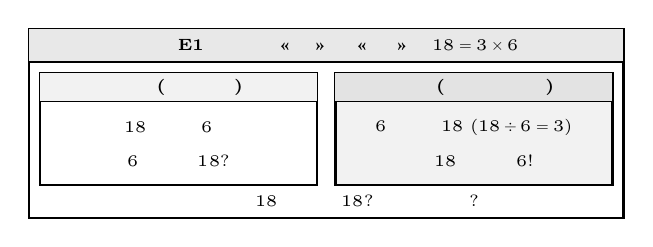
\begin{tikzpicture}[x=1cm, y=1cm, every node/.style={font=\fontsize{5.9pt}{7.8pt}\selectfont, text=black}]
  \draw[black, line width=0.9pt] (0,0) rectangle (7.55,2.40);
  \fill[gray!18] (0,1.98) rectangle (7.55,2.40);
  \draw[black, line width=0.6pt] (0,1.98) -- (7.55,1.98);
  \node at (3.775,2.19) {\textbf{បេសកកម្ម \en{E1}៖ អន្ទាក់ពាក្យ «តួចែក» និង «ពហុគុណ» លើ $18 = 3 \times 6$}};

  % Student A
  \draw[black, line width=0.8pt] (0.14,0.42) rectangle (3.66,1.84);
  \fill[gray!10] (0.14,1.48) rectangle (3.66,1.84);
  \draw[black, line width=0.5pt] (0.14,1.48) -- (3.66,1.48);
  \node at (1.90,1.66) {\textbf{សិស្ស ក (ច្រឡំទិសដៅពាក្យ)}};
  \node at (1.90,1.15) {$18$ ជា\textbf{តួចែក}នៃ $6$ ហើយ};
  \node at (1.90,0.72) {$6$ ជា\textbf{ពហុគុណ}នៃ $18$?};

  % Student B
  \draw[black, line width=0.95pt, fill=gray!10] (3.89,0.42) rectangle (7.41,1.84);
  \fill[gray!22] (3.89,1.48) rectangle (7.41,1.84);
  \draw[black, line width=0.55pt] (3.89,1.48) -- (7.41,1.48);
  \node at (5.65,1.66) {\textbf{សិស្ស ខ (ផ្ទៀងតាមអត្ថន័យចែកដាច់)}};
  \node at (5.65,1.15) {$6$ ជា\textbf{តួចែក}នៃ $18$ ($18\div 6=3$)};
  \node at (5.65,0.72) {រីឯ $18$ ជា\textbf{ពហុគុណ}នៃ $6$!};

  \node at (3.775,0.21) {\textbf{សំណួរ៖} តើតួចែកនៃ $18$ តូចជាងឬស្មើ $18$? ហើយមានប៉ុន្មានចំនួន?};
\end{tikzpicture}}

% ២. E2 Explore: គូកត្តាឥន្ទធនូនៃ 18 និងលក្ខណៈចែកដាច់នៃផលបូក/ដក (ទំ.១៨)
\newcommand{\figRainbowDIVTwoTwo}{%
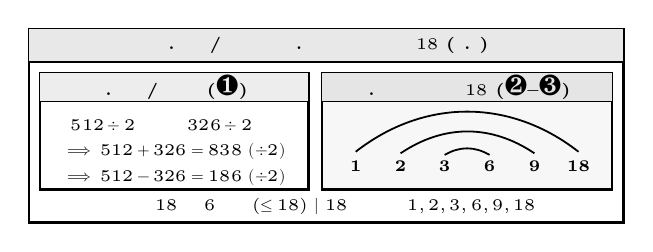
\begin{tikzpicture}[x=1cm, y=1cm, every node/.style={font=\fontsize{5.9pt}{7.7pt}\selectfont, text=black}]
  \draw[black, line width=0.9pt] (0,0) rectangle (7.55,2.46);
  \fill[gray!18] (0,2.04) rectangle (7.55,2.46);
  \draw[black, line width=0.6pt] (0,2.04) -- (7.55,2.04);
  \node at (3.775,2.25) {\textbf{១.២ ផលបូក/ដកចែកដាច់ និង ២. គូកត្តាឥន្ទធនូនៃតួចែក $18$ (ទំ.១៨)}};

  % Left: Sum/Diff divisibility
  \draw[black, line width=0.8pt] (0.14,0.42) rectangle (3.55,1.90);
  \fill[gray!14] (0.14,1.54) rectangle (3.55,1.90);
  \draw[black, line width=0.5pt] (0.14,1.54) -- (3.55,1.54);
  \node at (1.845,1.72) {\textbf{១.២ ផលបូក/ដកចែកដាច់ (\cnum{1})}};
  \node at (1.845,1.24) {$512\div 2$ ដាច់ និង $326\div 2$ ដាច់};
  \node at (1.845,0.90) {$\implies 512+326 = 838\ (\div 2)$};
  \node at (1.845,0.58) {$\implies 512-326 = 186\ (\div 2)$};

  % Right: Factor-pair rainbow of 18
  \draw[black, line width=0.8pt, fill=gray!6] (3.72,0.42) rectangle (7.41,1.90);
  \fill[gray!20] (3.72,1.54) rectangle (7.41,1.90);
  \draw[black, line width=0.5pt] (3.72,1.54) -- (7.41,1.54);
  \node at (5.565,1.72) {\textbf{២. គូកត្តារកតួចែកនៃ $18$ (\cnum{2}--\cnum{3})}};
  \node at (4.15,0.72) {$\mathbf{1}$};
  \node at (4.72,0.72) {$\mathbf{2}$};
  \node at (5.28,0.72) {$\mathbf{3}$};
  \node at (5.85,0.72) {$\mathbf{6}$};
  \node at (6.42,0.72) {$\mathbf{9}$};
  \node at (6.98,0.72) {$\mathbf{18}$};
  \draw[black, line width=0.65pt] (4.15,0.90) to[bend left=38] (6.98,0.90);
  \draw[black, line width=0.65pt] (4.72,0.88) to[bend left=34] (6.42,0.88);
  \draw[black, line width=0.65pt] (5.28,0.86) to[bend left=30] (5.85,0.86);

  \node at (3.775,0.21) {តួចែកនៃ $18$ មាន $6$ ចំនួន ($\le 18$) $\mid$ $18$ ជាពហុគុណនៃ $1, 2, 3, 6, 9, 18$};
\end{tikzpicture}}

% ៣. E4 Elaborate: លំហាត់គំរូ 3a+3 ចែកដាច់នឹង 3 និងគំរូតួចែក 8 / ពហុគុណ 16
\newcommand{\figModelsDIVTwoTwo}{%
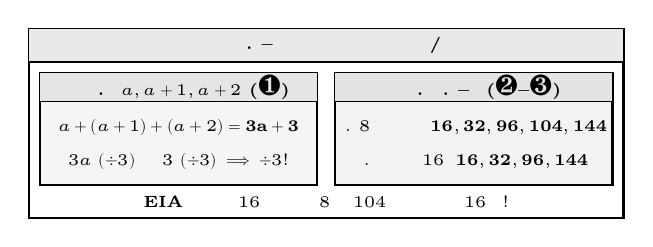
\begin{tikzpicture}[x=1cm, y=1cm, every node/.style={font=\fontsize{5.9pt}{7.7pt}\selectfont, text=black}]
  \draw[black, line width=0.9pt] (0,0) rectangle (7.55,2.40);
  \fill[gray!18] (0,1.98) rectangle (7.55,2.40);
  \draw[black, line width=0.6pt] (0,1.98) -- (7.55,1.98);
  \node at (3.775,2.19) {\textbf{លំហាត់គំរូ ទំ.១៨--១៩៖ ផលបូកបីចំនួនគត់តគ្នា និងតួចែក/ពហុគុណ}};

  % Left: a + (a+1) + (a+2)
  \draw[black, line width=0.8pt, fill=gray!8] (0.14,0.42) rectangle (3.66,1.84);
  \fill[gray!20] (0.14,1.48) rectangle (3.66,1.84);
  \draw[black, line width=0.5pt] (0.14,1.48) -- (3.66,1.48);
  \node at (1.90,1.66) {\textbf{គំរូ ១.២៖ $a, a+1, a+2$ (\cnum{1})}};
  \node at (1.90,1.15) {$a + (a+1) + (a+2) = \mathbf{3a + 3}$};
  \node at (1.90,0.72) {$3a\ (\div 3)$ និង $3\ (\div 3) \implies \div 3$!};

  % Right: Divisors of 8 vs Multiples of 16
  \draw[black, line width=0.85pt, fill=gray!10] (3.89,0.42) rectangle (7.41,1.84);
  \fill[gray!22] (3.89,1.48) rectangle (7.41,1.84);
  \draw[black, line width=0.5pt] (3.89,1.48) -- (7.41,1.48);
  \node at (5.65,1.66) {\textbf{គំរូ ២. ទំ.១៨--១៩ (\cnum{2}--\cnum{3})}};
  \node at (5.65,1.15) {ក. $8$ ជាតួចែកនៃ៖ $\mathbf{16, 32, 96, 104, 144}$};
  \node at (5.65,0.72) {ខ. ពហុគុណនៃ $16$៖ $\mathbf{16, 32, 96, 144}$};

  \node at (3.775,0.21) {\textbf{\en{EIA}៖} ពហុគុណនៃ $16$ ចែកដាច់នឹង $8$ តែ $104$ មិនមែនពហុគុណនៃ $16$ ទេ!};
\end{tikzpicture}}

% ៤. E5 Evaluate: សំណួរវិនិច្ឆ័យ A-D
\newcommand{\figExitDIVTwoTwo}{%
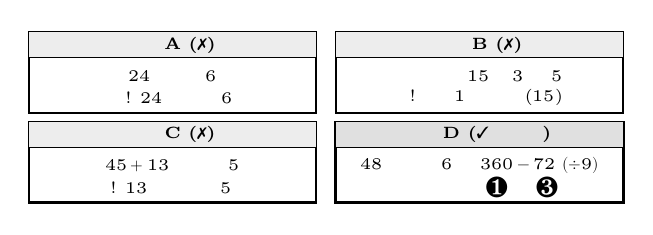
\begin{tikzpicture}[x=1cm, y=1cm, every node/.style={font=\fontsize{5.9pt}{7.6pt}\selectfont, text=black}]
  % Choice A
  \draw[black, line width=0.8pt] (0,1.14) rectangle (3.65,2.16);
  \fill[gray!14] (0,1.84) rectangle (3.65,2.16);
  \draw[black, line width=0.5pt] (0,1.84) -- (3.65,1.84);
  \node at (1.825,2.00) {\textbf{ជម្រើស \en{A} (\ding{55})}};
  \node at (1.825,1.61) {$24$ ជាតួចែកនៃ $6$};
  \node at (1.825,1.33) {ខុស! $24$ ជាពហុគុណនៃ $6$};

  % Choice B
  \draw[black, line width=0.8pt] (3.90,1.14) rectangle (7.55,2.16);
  \fill[gray!14] (3.90,1.84) rectangle (7.55,2.16);
  \draw[black, line width=0.5pt] (3.90,1.84) -- (7.55,1.84);
  \node at (5.725,2.00) {\textbf{ជម្រើស \en{B} (\ding{55})}};
  \node at (5.725,1.61) {តួចែកទាំងអស់នៃ $15$ គឺ $3$ និង $5$};
  \node at (5.725,1.33) {ខុស! ភ្លេច $1$ និងខ្លួនឯង ($15$)};

  % Choice C
  \draw[black, line width=0.8pt] (0,0) rectangle (3.65,1.02);
  \fill[gray!14] (0,0.70) rectangle (3.65,1.02);
  \draw[black, line width=0.5pt] (0,0.70) -- (3.65,0.70);
  \node at (1.825,0.86) {\textbf{ជម្រើស \en{C} (\ding{55})}};
  \node at (1.825,0.47) {$45 + 13$ ចែកដាច់នឹង $5$};
  \node at (1.825,0.19) {ខុស! $13$ មិនចែកដាច់នឹង $5$ ទេ};

  % Choice D (Correct)
  \draw[black, line width=1.05pt] (3.90,0) rectangle (7.55,1.02);
  \fill[gray!24] (3.90,0.70) rectangle (7.55,1.02);
  \draw[black, line width=0.6pt] (3.90,0.70) -- (7.55,0.70);
  \node at (5.725,0.86) {\textbf{ជម្រើស \en{D} (\ding{51} ត្រឹមត្រូវ)}};
  \node at (5.725,0.47) {$48$ ជាពហុគុណនៃ $6$ និង $360-72\ (\div 9)$};
  \node at (5.725,0.19) {ត្រូវតាមកូដហេតុផល \cnum{1} និង \cnum{3}};
\end{tikzpicture}}

\begin{document}
\fontsize{10pt}{15.2pt}\selectfont

% ============================================================================
% ក្បាលរដ្ឋបាល (Administrative Header — តាមគំរូ ls_plan.tex)
% ============================================================================
{\centering
  {\muol\fontsize{11pt}{16pt}\selectfont ព្រះរាជាណាចក្រកម្ពុជា\par}
  {\muol\fontsize{11pt}{16pt}\selectfont ជាតិ សាសនា ព្រះមហាក្សត្រ\par}
  \vspace{-3pt}{\khmflourish\par}
}

\vspace{1pt}
{\muol\fontsize{10pt}{15.5pt}\selectfont
មន្ទីរអប់រំ យុវជន និងកីឡា ខេត្តកំពង់ធំ\par
ការិយាល័យអប់រំ យុវជន និងកីឡា ស្រុកកំពង់ស្វាយ\par
អនុវិទ្យាល័យព្រះក្រសាំង\par}

\vspace{2pt}
{\centering{\muol\fontsize{11.5pt}{17pt}\selectfont កិច្ចតែងការបង្រៀន\par}}
\vspace{2pt}

% --- ព័ត៌មានទូទៅ ---
{\hspace*{2.8cm}\renewcommand{\arraystretch}{1.08}
\begin{tabular}{@{}l@{\hspace{0.35cm}}p{2.9cm}@{\hspace{0.15cm}}c@{\hspace{0.25cm}}l@{}}
  - & មុខវិជ្ជា & : & គណិតវិទ្យា ថ្នាក់ទី៧ (ពីជគណិត) \\
  - & ចំណងជើងមេរៀន & : & មេរៀនទី២៖ តួចែកនិងពហុគុណ \\
  - & ចំណងជើងរង & : & ១.២ ផលបូកនិងផលដកចែកដាច់ និង ២. តួចែកនិងពហុគុណ (ទំ.១៨--១៩) \\
  - & រយៈពេល & : & ១ ម៉ោងសិក្សា (៥០ នាទី) \\
  - & បង្រៀនដោយ & : & ហុក ប៊ុនថែន \\
  - & កាលបរិច្ឆេទ & : & ថ្ងៃសុក្រ ទី១៣ ខែវិច្ឆិកា ឆ្នាំ២០២៦ \\
\end{tabular}\par}

\vspace{2pt}

% --- I. វត្ថុបំណង ---
{\muol\fontsize{10pt}{15.5pt}\selectfont \enbf{I.} វត្ថុបំណង\par}
\vspace{1pt}
{\renewcommand{\arraystretch}{1.10}
\begin{tabular}{@{}p{0.55cm}@{}p{2.35cm}@{\hspace{0.15cm}}c@{\hspace{0.25cm}}p{14.95cm}@{}}
  \hfill\wcirc\hspace{0.2cm} & វិជ្ជាសម្បទា & : & សិស្សប្រាប់បានពីលក្ខណៈចែកដាច់នៃផលបូកនិងផលដក ព្រមទាំងប្រាប់បានពីនិយមន័យនិងទំនាក់ទំនងរវាងតួចែក និងពហុគុណនៃចំនួនគត់បានត្រឹមត្រូវ (ទំ.១៨--១៩) ។ \\
  \hfill\wcirc\hspace{0.2cm} & បំណិនសម្បទា & : & សិស្សបញ្ជាក់ភាពចែកដាច់នៃផលបូក/ផលដកដោយមិនបូកដកផ្ទាល់ និងរកគ្រប់តួចែកឬពហុគុណនៃចំនួនគត់តាមគូកត្តាលើសន្លឹកកិច្ចការបានត្រឹមត្រូវ ។ \\
  \hfill\wcirc\hspace{0.2cm} & ចរិយាសម្បទា & : & សិស្សមានភាពម៉ត់ចត់មិនច្រឡំទិសដៅពាក្យ «តួចែក» និង «ពហុគុណ» មិនរាយតួចែកខ្វះចន្លោះ និងសហការដោះស្រាយលំហាត់ជាក្រុមដោយសកម្ម ។ \\
\end{tabular}\par}

\vspace{2pt}

% --- II. សម្ភារៈឧបទេស ---
{\muol\fontsize{10pt}{15.5pt}\selectfont \enbf{II.} សម្ភារៈឧបទេស\par}
\vspace{1pt}
\hspace*{0.55cm}$\bullet$\ សៀវភៅសិក្សាគោលថ្នាក់ទី៧ (ទំ.១៨--១៩ និងទំ.២៤) ក្ដារខៀន ដីស/ហ្វឺត និង\textbf{សន្លឹកកិច្ចការសិស្សបំពេញចន្លោះ ស-ខ្មៅ} (កូដ \en{DIV22} ទំព័រ ១--២ សម្រាប់សិស្ស និងទំព័រ ៣ ប្លង់ក្ដារខៀន/ចម្លើយគ្រូ — គ្មានប្រើ \en{LCD})\par

\vspace{2pt}

% --- III. វិធីសាស្រ្តបង្រៀន ---
{\muol\fontsize{10pt}{15.5pt}\selectfont \enbf{III.} វិធីសាស្រ្តបង្រៀន\par}
\vspace{1pt}
{\renewcommand{\arraystretch}{1.08}
\begin{tabular}{@{}p{0.55cm}@{}p{2.35cm}@{\hspace{0.15cm}}c@{\hspace{0.25cm}}p{14.95cm}@{}}
  \hfill$\bullet$\hspace{0.2cm} & គោលវិធី & : & សិស្សមជ្ឈមណ្ឌល (សន្លឹកកិច្ចការបំពេញចន្លោះជាគោល + ការពិភាក្សាជាក្រុមតូច ៣ នាក់) \\
  \hfill$\bullet$\hspace{0.2cm} & យុទ្ធវិធីបង្រៀន & : & គំរូស្ថាបនានិយម \en{5Es} រួមបញ្ចូល \textbf{ការផ្គូផ្គងគូកត្តាឥន្ទធនូ (\en{Factor-Pair Rainbow})} និង \textbf{ការវិភាគទំនាក់ទំនងទៅមក (\en{Bidirectional Factor-Multiple Mapping})} \\
\end{tabular}\par}

\vspace{2pt}

% --- IV. ដំណើរការបង្រៀន ---
{\muol\fontsize{10pt}{15.5pt}\selectfont \enbf{IV.} ដំណើរការបង្រៀន\par}

{\renewcommand{\arraystretch}{1.14}
\begin{longtable}{|L{5.50cm}|L{7.90cm}|L{4.80cm}|}
\hline
\multicolumn{1}{|c|}{\cellcolor{headgray}\muol សកម្មភាពគ្រូ} &
\multicolumn{1}{c|}{\cellcolor{headgray}\muol ខ្លឹមសារមេរៀន} &
\multicolumn{1}{c|}{\cellcolor{headgray}\muol សកម្មភាពសិស្ស} \\
\hline
\endfirsthead

\hline
\multicolumn{1}{|c|}{\cellcolor{headgray}\muol សកម្មភាពគ្រូ} &
\multicolumn{1}{c|}{\cellcolor{headgray}\muol ខ្លឹមសារមេរៀន} &
\multicolumn{1}{c|}{\cellcolor{headgray}\muol សកម្មភាពសិស្ស} \\
\hline
\endhead

% ==================== ជំហានទី១ (2min) ====================
\stepheader{ជំហានទី១ \enbf{(}រដ្ឋបាលថ្នាក់\enbf{)}}
$\bullet$ ពិនិត្យវត្តមាន អនាម័យ និងសណ្ដាប់ធ្នាប់ថ្នាក់រៀន \par
$\bullet$ រៀបចំក្រុមតូច ៣ នាក់តាមតុ និងចែក\textbf{សន្លឹកកិច្ចការសិស្ស (\en{DIV22} ទំព័រ ១–២)}
&
$\bullet$ រដ្ឋបាលថ្នាក់ អនាម័យ និងវិន័យសិក្សា \par
$\bullet$ ចែកសន្លឹកកិច្ចការម្នាក់ ១ សន្លឹក សម្រាប់បំពេញតាមដំណាក់កាល \en{E1--E5}
&
$\circ$ ប្រធានថ្នាក់រាយការណ៍វត្តមានសិស្ស \par
$\circ$ ទទួលសន្លឹកកិច្ចការ សរសេរឈ្មោះ និងអង្គុយតាមក្រុម ៣ នាក់ \\
\hline

% ==================== ជំហានទី២ (9min: កំណែ <=3m + រំលឹក 3m + E1 3m) ====================
\stepheader{ជំហានទី២ \enbf{(}កិច្ចការផ្ទះ \enbf{+} ទំនាក់ទំនងមេរៀនថ្មី\enbf{)}}
\ditem \textbf{កំណែកិច្ចការផ្ទះ ($\le\text{\enbf{3\,min}}$)} \par
$\bullet$ ហៅសិស្សផ្ទៀងផ្ទាត់ចម្លើយលំហាត់ទំ.២៤ លេខ ២ និងលំហាត់ពង្រឹងលើក្ដារខៀនឆ្វេង
&
{\centering\redsub{កំណែកិច្ចការផ្ទះមេរៀនមុន (ទំ.២៤ លេខ ២ — $734\dbox 0$)}\par}
$\bullet$ \textbf{ក. ($\div 2$ និង $\div 5$)៖} គ្រប់លេខ $\dbox \in \{0,1,2,3,4,5,6,7,8,9\}$ (ព្រោះចុង $0$ ស្រាប់) \par
$\bullet$ \textbf{ខ. ($\div 3$ និង $\div 9$)៖} $7+3+4+\dbox+0=18 \implies \dbox = \mathbf{4}$ ($73\,440$)
&
$\circ$ ផ្ទៀងចម្លើយលេខ ២ និងកែចូលសៀវភៅ \\[3pt]

\ditem \textbf{រំលឹកមេរៀនទាក់ទង (\enbf{3min})} \par
$\bullet$ សួរ៖ «តើ $512$ និង $326$ ចែកដាច់នឹង $2$ ឬទេ? ហើយ $18$ អាចសរសេរជាផលគុណពីរចំនួនគត់អ្វីខ្លះ?»
&
{\centering\redsub{រំលឹកភាពចែកដាច់ និងផលគុណពីរកត្តា}\par}
$\bullet$ $512$ និង $326$ សុទ្ធតែជាចំនួនគត់គូ ដូច្នេះចែកដាច់នឹង $2$ \par
$\bullet$ $18 = 1\times 18 = 2\times 9 = 3\times 6$
&
$\circ$ ឆ្លើយ៖ «ចែកដាច់នឹង $2$ ទាំងពីរ ហើយ $18 = 1\times 18, 2\times 9, 3\times 6$!» \\[3pt]

\fiveE{E1 - Engage (3min)} \timenote{(កុំទាន់ផ្ដល់ចម្លើយ)} \par
\ditem \textbf{បេសកកម្មអន្ទាក់ពាក្យបច្ចេកទេស (\en{E1})}
&
\redsub{បេសកកម្ម \en{E1}៖ តើអ្នកណាប្រើពាក្យ «តួចែក» និង «ពហុគុណ» ត្រូវ?}
&
$\circ$ អានស្ថានភាពបញ្ហា \en{E1} \\[3pt]

$\bullet$ ឱ្យសិស្សពិភាក្សាជាគូលើសមីការ $18 = 3 \times 6$ រវាងសិស្ស ក និងសិស្ស ខ
&
$\bullet$ \textbf{សិស្ស ក៖} «$18$ ជាតួចែកនៃ $6$ ហើយ $6$ ជាពហុគុណនៃ $18$» \par
$\bullet$ \textbf{សិស្ស ខ៖} «$6$ ជាតួចែកនៃ $18$ ហើយ $18$ ជាពហុគុណនៃ $6$!»
&
$\circ$ ពិភាក្សាជាគូ និងគូស \ding{51} ក្នុងប្រអប់ \en{E1} \\[3pt]

&
\cfig{\figEngageDIVTwoTwo}
& \\
\hline

% ==================== ជំហានទី៣ (17min: E2 11m + E3 6m) ====================
\stepheader{ជំហានទី៣ \enbf{(}ខ្លឹមសារមេរៀនថ្មី\enbf{)}}
\fiveE{E2 - Explore (11min)} \par
$\bullet$ សរសេរចំណងជើងរង \textbf{១.២ លក្ខណៈចែកដាច់នៃផលបូកនិងផលដក} និង \textbf{២. តួចែកនិងពហុគុណ} \par
\ditem \textbf{សកម្មភាព ១៖ ផលបូកនិងផលដកចែកដាច់ (ទំ.១៨, \enbf{4.5min}, \en{E2-A})}
&
១.២ លក្ខណៈចែកដាច់នៃផលបូកនិងផលដក (ទំ.១៨) \par
$\bullet$ \textbf{ឧទាហរណ៍៖} $512\div 2$ ដាច់ និង $326\div 2$ ដាច់ $\implies$ ផលបូក $512+326 = \mathbf{838}$ ចែកដាច់នឹង $2$ ហើយផលដក $512-326 = \mathbf{186}$ ក៏ចែកដាច់នឹង $2$ ដែរ!
&
$\circ$ គណនាផលបូក $838$ និងផលដក $186$ ឃើញសុទ្ធតែគូ ($\div 2$) \\[3pt]

\ditem \textbf{សកម្មភាព ២៖ តួចែកនិងពហុគុណតាមគូកត្តាឥន្ទធនូ (ទំ.១៨--១៩, \enbf{6.5min}, \en{E2-B})} \par
$\bullet$ ឱ្យសិស្សបំពេញគូកត្តានៃ $18$ និង $100$ លើសន្លឹកកិច្ចការ \en{E2-B}
&
២. តួចែកនិងពហុគុណ (ទំ.១៨--១៩) \par
$\bullet$ \textbf{ឧទាហរណ៍ ១៖} $18 = 1\times 18 = 2\times 9 = 3\times 6 \implies$ \textbf{តួចែកនៃ $18$} គឺ $1, 2, 3, 6, 9, 18$ ហើយ $18$ ហៅថា \textbf{ពហុគុណ}នៃ $1, 2, 3, 6, 9, 18$ \par
$\bullet$ \textbf{ឧទាហរណ៍ ២៖} តួចែកនៃ $100$ គឺ $\mathbf{1, 2, 4, 5, 10, 20, 25, 50, 100}$ ($9$ ចំនួន)
&
$\circ$ ភ្ជាប់ធ្នូគូកត្តា ($1\leftrightarrow 100, 2\leftrightarrow 50, \dots$) មិនឱ្យភ្លេចតួចែក \\[3pt]

$\bullet$ ឱ្យសិស្សរាយពហុគុណដំបូងៗនៃ $7$ ដោយគុណនឹង $1, 2, 3, 4, \dots$
&
$\bullet$ \textbf{ឧទាហរណ៍ ៣ (ទំ.១៨)៖} ពហុគុណនៃ $7$ គឺ $7\times 1 = 7,\ 7\times 2 = 14,\ 7\times 3 = 21,\ 7\times 4 = 28,\ 7\times 5 = 35, \dots$ (មានច្រើនរាប់មិនអស់)
&
$\circ$ គុណបន្តបន្ទាប់រកពហុគុណនៃ $7$ \\[3pt]

&
\cfig{\figRainbowDIVTwoTwo}
& \\[3pt]

% --- E3 Explain (6min) ---
\fiveE{E3 - Explain (6min)} \par
$\bullet$ ដឹកនាំសិស្សសង្ខេបវិធាន «ជាទូទៅ» និង «សម្គាល់» (ទំ.១៨) លើ \en{E3}
&
$\bullet$ \textbf{សង្ខេបខ្លឹមសារគោល (ទំ.១៨)៖} \par
\hspace*{0.15cm}១) បើតួនីមួយៗនៃផលបូក ឬផលដក ចែកដាច់នឹងចំនួន $k$ ដូចគ្នា នោះ\graybox{ផលបូក ឬផលដក}របស់វា ក៏ចែកដាច់នឹង $k$ ដែរ \par
\hspace*{0.15cm}២) បើ $a$ ចែកដាច់នឹង $b$ នោះ $b$ ជា\graybox{តួចែក}នៃ $a$ $\iff a$ ជា\graybox{ពហុគុណ}នៃ $b$
&
$\circ$ បំពេញប្រអប់សង្ខេបវិធានទាំងពីរលើ \en{E3} \\[3pt]

$\bullet$ បញ្ជាក់ចំណុច\textbf{សម្គាល់ (ទំ.១៨)} អំពីចំនួនតួចែក និងចំនួនពហុគុណ
&
$\bullet$ \textbf{សម្គាល់ (ទំ.១៨)៖} គ្រប់ចំនួនគត់ធម្មជាតិ $n$ មានតួចែក $1$ និងខ្លួនឯងជានិច្ច ។ ចំនួនតួចែកនៃ $n$ មានកំណត់ ($\le n$) រីឯពហុគុណនៃ $n$ មានច្រើនរាប់មិនអស់ ។
&
$\circ$ កត់សម្គាល់ភាពខុសគ្នារវាងតួចែក (មានកំណត់) និងពហុគុណ \\[3pt]

$\bullet$ ភ្ជាប់\textbf{ធនាគារហេតុផល \cnum{1}} លើក្ដារខៀន និងសន្លឹកកិច្ចការ
&
\textbf{ធនាគារហេតុផល (\en{Warrant Bank})៖} \par
\cnum{1} \textbf{ផលបូក/ដកចែកដាច់៖} $a\div k$ ដាច់ និង $b\div k$ ដាច់ $\implies (a\pm b)\div k$ ដាច់
&
$\circ$ ផ្ទៀងលេខកូដ \cnum{1} លើសន្លឹកកិច្ចការ \\[3pt]

$\bullet$ ភ្ជាប់\textbf{ធនាគារហេតុផល \cnum{2}} សម្រាប់លក្ខណៈតួចែក
&
\cnum{2} \textbf{លក្ខណៈតួចែក៖} គ្រប់ចំនួន $n$ មានតួចែក $1$ និងខ្លួនឯង ($n$) ជានិច្ច (តួចែក $\le n$)
&
$\circ$ ផ្ទៀងលេខកូដ \cnum{2} លើសន្លឹកកិច្ចការ \\[3pt]

$\bullet$ ភ្ជាប់\textbf{ធនាគារហេតុផល \cnum{3}--\cnum{4}} សម្រាប់ពហុគុណ និងគូកត្តាឥន្ទធនូ
&
\cnum{3} \textbf{ពហុគុណ៖} $a$ ជាពហុគុណនៃ $b$ កាលណា $a = b\times q$ (ចែកដាច់គ្មានសំណល់) \par
\cnum{4} \textbf{គូកត្តាឥន្ទធនូ៖} រាយតួចែកជាគូផលគុណពីក្រៅចូលក្នុង ដើម្បីកុំឱ្យបាត់តួចែក
&
$\circ$ ផ្ទៀងលេខកូដ \cnum{3}--\cnum{4} លើសន្លឹកកិច្ចការ \\
\hline

% ==================== ជំហានទី៤ (20min: E4 10m + E5 10m) ====================
\stepheader{ជំហានទី៤ \enbf{(}ពង្រីកចំណេះដឹង\enbf{)}}
\fiveE{E4 - Elaborate (10min)} \par
\ditem \textbf{លំហាត់គំរូ ១.២ (ទំ.១៨) និងលំហាត់គំរូ ២. (ទំ.១៨--១៩)} \par
$\bullet$ ឱ្យសិស្សដោះស្រាយលំហាត់គំរូទំ.១៨ (ផលបូកបីចំនួនគត់តគ្នា $a, a+1, a+2$) លើ \en{E4}
&
{\muol លំហាត់គំរូ} \textbf{(សៀវភៅគោល ទំ.១៨--១៩)៖} \par
$\bullet$ \textbf{គំរូ ១.២ (ទំ.១៨)៖} ផលបូក $a + (a+1) + (a+2) = \graybox{$3a + 3$}$ ។ ដោយ $3a$ ចែកដាច់នឹង $3$ ហើយ $3$ ចែកដាច់នឹង $3$ នោះ $3a+3$ ចែកដាច់នឹង $3$ (\cnum{1})
&
$\circ$ បូកតួដូចគ្នាបាន $3a+3$ រួចសំអាងលេខកូដ \cnum{1} \\[3pt]

$\bullet$ ឱ្យសិស្សដោះស្រាយលំហាត់គំរូទំ.១៨--១៩ លើចំនួន $12, 16, 28, 32, 41, 96, 104, 126, 144$
&
$\bullet$ \textbf{គំរូ ២. (ទំ.១៨--១៩)៖} ក. $8$ ជាតួចែកនៃ៖ \graybox{$16, 32, 96, 104, 144$} (\cnum{2}) \par
\hspace*{0.2cm}ខ. ពហុគុណនៃ $16$ គឺ៖ \graybox{$16, 32, 96, 144$} (\cnum{3})
&
$\circ$ ជ្រើសរើសចំនួនដែលចែកដាច់នឹង $8$ និងនឹង $16$ \\[3pt]

&
\cfig{\figModelsDIVTwoTwo}
& \\[3pt]

$\bullet$ សួរសំណួរឆ្លុះបញ្ចាំង \textbf{\en{EIA Looking-Back} (1min)} បំបែកអន្ទាក់ទាញច្រាសផលបូក
&
\textbf{\en{EIA Looking-Back}៖} «ផលបូក $7 + 5 = 12$ ចែកដាច់នឹង $2$ — តើ $7$ និង $5$ ចែកដាច់នឹង $2$ ដែរឬទេ?» ($\to$ ទេ! ច្រាសនៃទ្រឹស្ដីបទ \cnum{1} មិនពិតជានិច្ចទេ!)
&
$\circ$ ឆ្លុះបញ្ចាំងថា $7$ និង $5$ ជាចំនួនសេស មិនចែកដាច់នឹង $2$ ទេ \\[3pt]

% --- E5 Evaluate (10min) ---
\fiveE{E5 - Evaluate (10min)} \par
\ditem \textbf{ប្រតិបត្តិជាក្រុមតូច ៣ នាក់ (4min, សន្លឹកកិច្ចការ \en{E5})} \par
$\bullet$ ឱ្យក្រុមសិស្សដោះស្រាយប្រតិបត្តិទំ.១៨ (បំពេញខ្ទង់ឱ្យចែកដាច់នឹង $9$)
&
{\muol លំហាត់ប្រតិបត្តិ} \textbf{(សៀវភៅគោល ទំ.១៨ និង ទំ.១៩)៖} \par
$\bullet$ \textbf{ប្រតិបត្តិ ទំ.១៨ ($\div 9$)៖} ក. $3\mathbf{6}0 + 16\mathbf{2}$ \quad ខ. $40\mathbf{5} - 2\mathbf{7}0$ (ធ្វើឱ្យតួនីមួយៗចែកដាច់នឹង $9$ តាម \cnum{1})
&
$\circ$ បំពេញប្រអប់ឱ្យតួនីមួយៗចែកដាច់នឹង $9$ \\[3pt]

$\bullet$ ឱ្យក្រុមសិស្សដោះស្រាយប្រតិបត្តិទំ.១៩ (រកពហុគុណនៃ $6$ និងរាយគ្រប់តួចែក)
&
$\bullet$ \textbf{ប្រតិបត្តិ ទំ.១៩៖} ក. ពហុគុណនៃ $6$ គឺ $\mathbf{30, 48, 66}$ (\cnum{3}) \par
\hspace*{0.15cm}ខ. តួចែកនៃ $15$៖ $\{1,3,5,15\}$; នៃ $24$៖ $\{1,2,3,4,6,8,12,24\}$; នៃ $68$៖ $\{1,2,4,17,34,68\}$; នៃ $120$៖ $\{1,2,3,4,5,6,8,10,12,15,20,24,30,40,60,120\}$ (\cnum{4})
&
$\circ$ រាយតួចែកតាមគូកត្តាឥន្ទធនូដោយគ្មានបាត់ចំនួន \\[3pt]

$\bullet$ ឱ្យក្រុមសិស្សផ្ទៀងផ្ទាត់និង\textbf{បិទបេសកកម្ម \en{E1} (2min)}
&
$\bullet$ \textbf{បិទបេសកកម្ម \en{E1}៖} \textbf{សិស្ស ខ} ត្រឹមត្រូវ! $6$ ជា\textbf{តួចែក}នៃ $18$ ហើយ $18$ ជា\textbf{ពហុគុណ}នៃ $6$ (\cnum{2}, \cnum{3}) ។
&
$\circ$ បិទបេសកកម្ម \en{E1} ឃើញសិស្ស ខ ត្រឹមត្រូវ \\[3pt]

\ditem \textbf{សំណួរវិនិច្ឆ័យ \en{A--D} និងសំបុត្រចេញ (4min)} \par
$\bullet$ សរសេរជម្រើស \en{A--D} លើក្ដារខៀន
&
{\centering\textbf{សំណួរវិនិច្ឆ័យ \en{A--D}៖ តើប្រយោគមួយណាត្រឹមត្រូវ?}\par}
&
$\circ$ ពិនិត្យជម្រើសទាំង ៤ តាមកូដហេតុផល \cnum{1}--\cnum{4} \\[3pt]

$\bullet$ ឱ្យសិស្សគូសរង្វង់លើសន្លឹកកិច្ចការ និងលើកម្រាមដៃ ១--៤ ព្រមគ្នា
&
$\bullet$ វិភាគកំហុសក្នុងជម្រើស \en{A} (ត្រឡប់ពាក្យ), \en{B} (ភ្លេច $1, 15$), \en{C} ($13\not\div 5$)
&
$\circ$ គូសរង្វង់លើសន្លឹកកិច្ចការ និងលើកម្រាមដៃ ៤ (\textbf{ជម្រើស \en{D}}) \\[3pt]

&
\cfig{\figExitDIVTwoTwo}
& \\[3pt]

$\bullet$ បញ្ជាក់ចម្លើយត្រូវ (\textbf{ជម្រើស \en{D}}) និងឱ្យបំពេញ\textbf{សំបុត្រចេញ ៦០ វិនាទី}
&
$\bullet$ \textbf{សំបុត្រចេញ៖} រាយតួចែកទាំងអស់នៃ $20$ តាមគូកត្តា ($\implies \mathbf{1, 2, 4, 5, 10, 20}$) ។
&
$\circ$ បំពេញតួចែកទាំង $6$ នៃ $20$ មុនបញ្ចប់ម៉ោង \\
\hline

% ==================== ជំហានទី៥ (<=2min) ====================
\stepheader{ជំហានទី៥ \enbf{(}កិច្ចការផ្ទះ \enbf{+} បណ្ដាំផ្ញើ\enbf{)}}
\timenote{ចំណាយពេលឱ្យតិចបំផុតកុំឱ្យលើស 2min} \par
$\bullet$ ណែនាំប្រអប់\textbf{កិច្ចការផ្ទះ}លើសន្លឹកកិច្ចការទំព័រ ២ (សៀវភៅគោល ទំ.២៤ លេខ ១ និង លេខ ៣)
&
{\centering{\muol កិច្ចការផ្ទះ} \textbf{(សៀវភៅគោល ទំ.២៤ លេខ ១ និង លេខ ៣)}\par} \par
$\bullet$ \textbf{លេខ ១៖} ចូរបញ្ជាក់ថា៖ ក. $78+120$ ($\div 2$) \quad ខ. $4\,140-720$ ($\div 3$) \par
\hspace*{0.25cm}គ. $165+270$ ($\div 5$) \quad ឃ. $5\,130-342$ ($\div 9$) \par
$\bullet$ \textbf{លេខ ៣៖} គេមានចំនួន $660, 540, 645$ និង $610$ ។ តើចំនួនណាខ្លះជាពហុគុណនៃ $30$?
&
$\circ$ គូសចំណាំលំហាត់ទំ.២៤ លេខ ១ និង លេខ ៣ \\[3pt]

$\bullet$ ផ្ដាំផ្ញើឱ្យអានមុនចំណុច ៣. ចំនួនបឋម (ទំ.១៩) សម្រាប់ម៉ោងក្រោយ
&
$\bullet$ \textbf{បណ្ដាំផ្ញើ៖} អានមុន \textbf{៣. ចំនួនបឋម} (សៀវភៅគោល ទំ.១៩) និងសាកល្បងរកតួចែកនៃ $5, 14, 15, 23$ ។
&
$\circ$ កត់ត្រាបណ្ដាំផ្ញើ ទុកសន្លឹកកិច្ចការក្នុងសៀវភៅ និងជម្រាបលាគ្រូ \\
\hline
\end{longtable}}

\vspace{6pt}
% --- ហត្ថលេខា (កាលបរិច្ឆេទត្រូវគ្នា ១០០% នឹងខាងលើ) ---
{\centering
\hspace*{5.2cm}\begin{minipage}{11.5cm}
  \centering
  ថ្ងៃសុក្រ ៤កើត ខែកត្តិក ឆ្នាំមមី អដ្ឋស័ក ពុទ្ធសករាជ ២៥៧០\par
  កំពង់ស្វាយ, ថ្ងៃទី១៣ ខែវិច្ឆិកា ឆ្នាំ២០២៦\par
  \vspace{2pt}
  {\muol គ្រូបង្រៀន\par}
  \vspace{32pt}
  \hfill{\muol ហុក ប៊ុនថែន}\hspace*{1.4cm}
\end{minipage}\par}

\end{document}
